% !TEX root =  ../main.tex
\section{Root}
\subsection{Definition}

\subsubsection{Signature} \cstr{root(s : set<VM>)}
\begin{itemize}
\item \cstr{s} : an non-empty set of VMs for a meaningful constraint. VMs not in the \st{Running} state are ignored.
\end{itemize}

The \cstr{root} constraint forces each running VM in \cstr{s} to not move from its current location.
%
This constraint only restricts the placement of running VMs with regards to a previous placement.
As a result, it is not possible to state for the satisfaction of one \cstr{root} constraint before a reconfiguration occurred.

%\classification{root}{application administrator,datacenter administrator}{VM placement}{VM-to-server placement,Performance,Resource management}

\classification{root}{application administrator,datacenter administrator}{VM placement}{VM-to-server placement,Performance,Resource management}

\subsubsection{Usage}

The \cstr{root} constraint is mostly used to disallow the relocation of VMs when it is not possible or tolerated.
Typically, a running VM may be attached to a peculiar device such as a filesystem or a PCI device on its host.
In this setting, the relocation of the VM may not  maintain this link and should not be performed for reliability reasons.
An application administrator may then use a \cstr{root} constraint on this constraint to prevent from relocation.
In addition, an application administrator may disallow the relocation of his VMs to prevent from the temporary performance loss that occur during this action.

Another possible usage is to disallow VMs relocation when the infrastructure or the underlying hypervisor does
not support it. In this setting, the datacenter administrator may use a \cstr{root} constraint on all the VMs to disallow their relocation.

\subsubsection{Example}

Figure~\ref{fig: root} depicts a sample reconfiguration between a source and a destination configuration. In this example, the following \cstr{root} constraints were considered:

\begin{reconfiguration}
\centering
\begin{minipage}[b]{0.40\textwidth}
\begin{lstlisting}
N1: VM1 VM2
N2: VM3 VM5
?: VM4
\end{lstlisting}
\end{minipage}
\begin{minipage}[b]{2cm}
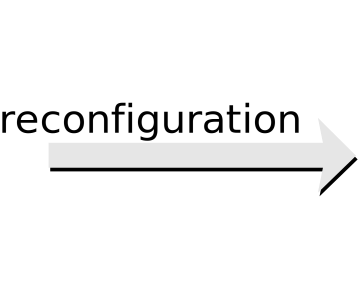
\includegraphics[width=2cm]{img/arrow_reconfiguration}
\end{minipage}
\begin{minipage}[b]{0.40\textwidth}
\begin{lstlisting}
N1: VM1 VM4
N2: VM3 VM2
?: VM5
\end{lstlisting}
\end{minipage}
\caption{A reconfiguration motivated by \cstr{root} constraints.}\label{fig: root}
\end{reconfiguration}

\begin{itemize}
\item \cstr{root(\{VM1,VM3\})}. This constraint is satisfied as none of the VMs were relocated during the reconfiguration
\item \cstr{root(\{VM4, VM5\})}. This constraint is satisfied as \cstr{VM4} is not running in the initial configuration while \cstr{VM5} is no longer running in the destination configuration. The constraint ignores then these VMs.
\item \cstr{root(\{VM2\})}. This constraint is not satisfied as \cstr{VM2} has been relocated from \cstr{N1} to \cstr{N2} during the reconfiguration process.
\end{itemize}



\fullVersion{
\subsection{Model}

This constraint is modeled using a domain restriction on the demanding slice associated to each of the running VMs.

\begin{equation*}
\begin{split}
\forall S \subseteq \mathcal{V},\ root(S) \triangleq &\\
&   \forall v_i \in V, d_i^h = c_i^h | \exists d_i^h \in \mathcal{D} , c_i^h \in \mathcal{C}
\end{split}
\end{equation*}

\subsection{Violation Detection}

\subsection{Availability}
\subsubsection{In {\btrp}} This constraint is available in {\btrp} since the version 2.0 using the name \texttt{Root}.
Using the global constraint catalog, the assignment of the d-slice placement variable is performed using a \emph{eq} constraint.

\begin{equation*}
\begin{split}
\forall S \subseteq \mathcal{V},\ root(S) \triangleq &\\
&   \forall v_i \in V, eq(d_i^h, c_i^h) | \exists d_i^h \in \mathcal{D} , c_i^h \in \mathcal{C}
\end{split}
\end{equation*}
}


\subsection{See also}

\subsubsection{Related Constraints}
\begin{itemize}
\item \cstrref{fence}: The \cstr{root} constraint can be emulated using a \cstr{fence} constraint when its user knows the current host of the specified VMs. For each VM, the list of servers given in the \cstr{fence} constraint is a singleton only composed of the current hosting server.
\end{itemize}

\printListOfInheritance{root}